\documentclass[12pt, titlepage]{article}

\usepackage{xcolor} % for different colour comments
\usepackage{tabto}
\usepackage{mdframed}
\mdfsetup{nobreak=true}
\usepackage{xkeyval}
\usepackage{tabularx}
\usepackage{booktabs}
\usepackage{hyperref}
\hypersetup{
    colorlinks,
    citecolor=black,
    filecolor=black,
    linkcolor=red,
    urlcolor=blue
}
\usepackage[skip=2pt, labelfont=bf]{caption}
\usepackage{titlesec}
\usepackage{graphicx}
\graphicspath{ {image/} }



%% the following adds another section level by redefining the paragraph
%% source:  http://tex.stackexchange.com/questions/60209/how-to-add-an-extra-level-of-sections-with-headings-below-subsubsection
\setcounter{secnumdepth}{4}

\titleformat{\paragraph}
{\normalfont\normalsize\bfseries}{\theparagraph}{1em}{}
\titlespacing*{\paragraph}
{0pt}{3.25ex plus 1ex minus .2ex}{1.5ex plus .2ex}


%% Comments
\newif\ifcomments\commentstrue

\ifcomments
\newcommand{\authornote}[3]{\textcolor{#1}{[#3 ---#2]}}
\newcommand{\todo}[1]{\textcolor{red}{[TODO: #1]}}
\else
\newcommand{\authornote}[3]{}
\newcommand{\todo}[1]{}
\fi

\newcommand{\wss}[1]{\authornote{magenta}{SS}{#1}}
\newcommand{\ds}[1]{\authornote{blue}{DS}{#1}}



%% The following are used for pretty printing of events and requirements
\makeatletter

\define@cmdkey      [TP] {test}     {name}       {}
\define@cmdkey      [TP] {test}     {desc}       {}
\define@cmdkey      [TP] {test}     {type}       {}
\define@cmdkey      [TP] {test}     {init}       {}
\define@cmdkey      [TP] {test}     {input}      {}
\define@cmdkey      [TP] {test}     {output}     {}
\define@cmdkey      [TP] {test}     {pass}       {}
\define@cmdkey      [TP] {test}     {user}       {}


\newcommand{\getCurrentSectionNumber}{%
  \ifnum\c@section=0 %
  \thechapter
  \else
  \ifnum\c@subsection=0 %
  \thesection
  \else
  \ifnum\c@subsubsection=0 %
  \thesubsection
  \else
  \thesubsubsection
  \fi
  \fi
  \fi
}

\newcounter{TestNum}

\@addtoreset{TestNum}{section}
\@addtoreset{TestNum}{subsection}
\@addtoreset{TestNum}{subsubsection}

\newcommand{\testauto}[1]{
\setkeys[TP]{test}{#1}
\refstepcounter{TestNum}
\begin{mdframed}[linewidth=1pt]
\begin{tabularx}{\textwidth}{@{}p{3cm}X@{}}
{\bf Test \getCurrentSectionNumber.\theTestNum:} & {\bf \cmdTP@test@name}\\[\baselineskip]
{\bf Description:} & \cmdTP@test@desc\\[0.5\baselineskip]
{\bf Type:} & \cmdTP@test@type\\[0.5\baselineskip]
{\bf Initial State:} & \cmdTP@test@init\\[0.5\baselineskip]
{\bf Input:} & \cmdTP@test@input\\[0.5\baselineskip]
{\bf Output:} & \cmdTP@test@output\\[0.5\baselineskip]
{\bf Pass:} & \cmdTP@test@pass
\end{tabularx}
\end{mdframed}
}

\newcommand{\testmanual}[1]{
\setkeys[TP]{test}{#1}
\refstepcounter{TestNum}
\begin{mdframed}[linewidth=1pt]
\begin{tabularx}{\textwidth}{@{}p{3cm}X@{}}
{\bf Test \getCurrentSectionNumber.\theTestNum:} & {\bf \cmdTP@test@name}\\[\baselineskip]
{\bf Description:} & \cmdTP@test@desc\\[0.5\baselineskip]
{\bf Type:} & \cmdTP@test@type\\[0.5\baselineskip]
{\bf Tester(s):} & \cmdTP@test@user\\[0.5\baselineskip]
{\bf Pass:} & \cmdTP@test@pass
\end{tabularx}
\end{mdframed}
}


\makeatother


\begin{document}
\title{\bf Physics-Based Chipmunk2D Game\\[\baselineskip]\Large Test Plan}
\author{Steven Palmer\\$\langle$palmes4$\rangle$\\Emaad Fazal\\$\langle$fazale$\rangle$\\Chao Ye\\$\langle$yec6$\rangle$}
\date{\today}
	
\maketitle

\pagenumbering{roman}
\tableofcontents


\begin{table}[bp]
\caption*{\bf Revision History}
\begin{tabularx}{\textwidth}{p{3.5cm}p{2cm}X}
\toprule {\bf Date} & {\bf Version} & {\bf Notes}\\
\midrule
October 25, 2015 & 1.0 & Created document\\
\bottomrule
\end{tabularx}
\end{table}

\newpage

\pagenumbering{arabic}

\section{Overview}
The purpose of this document is to provide a detailed plan for the testing of our game.  The following brief outline gives and overview of what is covered in this document:

\begin{itemize}
  \item A proof of concept test is described in \hyperref[sec:poc]{\S\ref*{sec:poc}}.
  \item System testing is separated into game mechanics testing and game design testing.  The set of tests that will be used in testing the system is described in \hyperref[sec:testing]{\S\ref*{sec:testing}}.
  \item The set of tests that will be used to ensure that the software requirements specifications are met is described in \hyperref[sec:reqtesting]{\S\ref*{sec:reqtesting}}.
  \item A timeline of the test plan is given in \hyperref[sec:timeline]{\S\ref*{sec:timeline}}.  
\end{itemize}


\subsection{Constants}
Constants used in this document are listed in \hyperref[tab:constants]{Table~\ref*{tab:constants}}.
\begin{table}[ht]
\caption{List of constants} \label{tab:constants}
\begin{tabularx}{\textwidth}{p{3cm}p{2cm}X}
\toprule {\bf Constant} & {\bf Value} & {\bf Description}\\
\midrule
$\alpha$ & 5.0 & Walk speed\\
$\beta$ & 3.0 & Run speed factor: run speed = $\alpha \times \beta$\\
\bottomrule
\end{tabularx}
\end{table}
\subsection{Terminology}
Terminology used in this document are listed in \hyperref[tab:terminology]{Table~\ref*{tab:terminology}}.
\begin{table}[ht]
\caption{List of terminology} \label{tab:terminology}
\begin{tabularx}{\textwidth}{p{3cm}X}
\toprule {\bf Term} & {\bf Definition}\\
\midrule
\bottomrule
\end{tabularx}
\end{table}

\section{Proof of Concept Testing}
\label{sec:poc}
Before any serious development of the game begins, a proof of concept test will be carried out to show that the undertaking is feasible.  The remainder of this section provides detail on what will be used as a proof of concept test.

\subsection{Significant Risks}
The successful completion of the project depends on overcoming the following significant risks:
\begin{enumerate}
  \item In order to use the Chipmunk2D library it must first be successfully compiled.  Since we intend for the game to be compatible with Windows 7, Mac OS X, and Ubuntu, there is a significant risk for the project to fail if compilation is not achieved on all three operating systems.
  \item Chipmunk2D is a large library and its use is not straight forward.  Successful implementation of the library features is crucial to the success of the project and the failure of this poses another significant risk.
\end{enumerate}


\subsection{Demonstration Plan}

For a proof of concept test we will produce a working prototype that can be run on Windows 7, Mac OS X, and Ubuntu.  The prototype will consist of a game demo that implements gravity and collision detection provided by the Chipmunk2D library.  Rudimentary graphics will be used for the prototype since the scope is limited only to demonstrating that the identified risks can be overcome.

The prototype will consist of a small room in which a hero character and enemies exist.  The room will be bounded by a floor below and walls on the left and right, all of which the hero and enemies cannot pass through.  The room will contain platforms which the hero and enemies cannot pass through from above, but may pass through from below when jumping.  A rough idea of the room is given in \hyperref[fig:room]{Figure~\ref*{fig:room}}.

\begin{figure}[ht]
\begin{center}
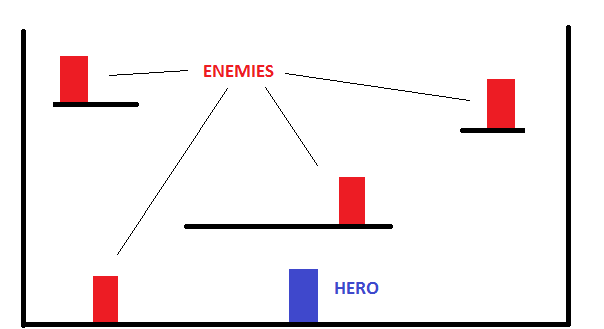
\includegraphics[width=0.75\textwidth]{demo}
\caption{Proof of concept sketch} \label{fig:room}
\end{center}
\end{figure}

The hero character will be represented by a blue rectangle and will be controlled by the user in the following ways:

\begin{itemize}
  \item The hero moves left and right using the 'a' and 'd' keys respectively
  \item The hero jumps by pressing the 'space' key
  \item The hero shoots a projectile in the direction of the mouse cursor by left-clicking
\end{itemize}

Enemies will be represented by red rectangles and will not have any programmed AI (they will not move or attack).  The hero will be able to attack enemies with a projectile, which will knock them back when they are hit.  The hero and all enemies will be subject to gravity and will free-fall when there is no platform or boundary under them.

\subsection{Proof of Concept Test}

\testmanual{
    name = Proof of Concept,
    desc = Tests whether significant risks to the completion of the project can be overcome,
    type = {Proof of Concept (manual)},
    user = Game developers,
    pass = Successful development of a small demonstration which makes use of the Chipmunk2D physics engine
}


\section{System Testing}
\label{sec:testing}
\subsection{Game Mechanics Testing}
\label{sec:mechanicstesting}
Automated unit testing will be used as the primary method for testing the game mechanics.  The test cases that will be used are outlined in the remainder of this section.
\subsubsection{Input Testing}
The following tests will ensure that user inputs are processed properly.

\testauto{
    name = {Walk left, started from stationary},
    desc = Tests if the hero walks left when the corresponding input is received when the hero is initially stationary,
    type = {Unit Test (dynamic, automated)},
    init = Custom game state with hero object having x-velocity of zero,
    input = Keyboard function called with simulated left key down stroke,
    output = Hero x-velocity (side-effect),
    pass = Hero x-velocity is $-\alpha$
}

\testauto{
    name = {Walk left, started from walking left},
    desc = Tests if the hero walks left when the corresponding input is received when the hero is initially walking left,
    type = {Unit Test (dynamic, automated)},
    init = Custom game state with hero object having x-velocity of $-\alpha$,
    input = Keyboard function called with simulated left key down stroke,
    output = Hero x-velocity (side-effect),
    pass = Hero x-velocity is $-\alpha$
}

\testauto{
    name = {Walk left, started from running left},
    desc = Tests if the hero walks left when the corresponding input is received when the hero is initially running left,
    type = {Unit Test (dynamic, automated)},
    init = Custom game state with hero object having x-velocity of $-\beta\times\alpha$,
    input = Keyboard function called with simulated left key down stroke,
    output = Hero x-velocity (side-effect),
    pass = Hero x-velocity is $-\alpha$
}

\testauto{
    name = {Run left, started from stationary},
    desc = Tests if the hero runs left when the corresponding input is received when the hero is initially stationary,
    type = {Unit Test (dynamic, automated)},
    init = Custom game state with hero object having x-velocity of zero,
    input = Keyboard function called with simulated left key down stroke modified by the shift key,
    output = Hero x-velocity (side-effect),
    pass = Hero x-velocity is $-\beta\times\alpha$
}

\testauto{
    name = {Run left, started from walking left},
    desc = Tests if the hero runs left when the corresponding input is received when the hero is initially walking left,
    type = {Unit Test (dynamic, automated)},
    init = Custom game state with hero object having x-velocity of $-\alpha$,
    input = Keyboard function called with simulated left key down stroke modified by the shift key,
    output = Hero x-velocity (side-effect),
    pass = Hero x-velocity is $-\beta\times\alpha$
}

\testauto{
    name = {Run left, started from running left},
    desc = Tests if the hero runs left when the corresponding input is received when the hero is initially running left,
    type = {Unit Test (dynamic, automated)},
    init = Custom game state with hero object having x-velocity of $-\beta\times\alpha$,
    input = Keyboard function called with simulated left key down stroke modified by the shift key,
    output = Hero x-velocity (side-effect),
    pass = Hero x-velocity is $-\beta\times\alpha$
}

\testauto{
    name = {Walk right, started from stationary},
    desc = Tests if the hero walks right when the corresponding input is received when the hero is initially stationary,
    type = {Unit Test (dynamic, automated)},
    init = Custom game state with hero object having x-velocity of zero,
    input = Keyboard function called with simulated right key down stroke,
    output = Hero x-velocity (side-effect),
    pass = Hero x-velocity is $\alpha$
}

\testauto{
    name = {Walk right, started from walking right},
    desc = Tests if the hero walks right when the corresponding input is received when the hero is initially walking right,
    type = {Unit Test (dynamic, automated)},
    init = Custom game state with hero object having x-velocity of $\alpha$,
    input = Keyboard function called with simulated right key down stroke,
    output = Hero x-velocity (side-effect),
    pass = Hero x-velocity is $\alpha$
}

\testauto{
    name = {Walk right, started from running right},
    desc = Tests if the hero walks right when the corresponding input is received when the hero is initially running right,
    type = {Unit Test (dynamic, automated)},
    init = Custom game state with hero object having x-velocity of $\beta\times\alpha$,
    input = Keyboard function called with simulated right key down stroke,
    output = Hero x-velocity (side-effect),
    pass = Hero x-velocity is $\alpha$
}

\testauto{
    name = {Run right, started from stationary},
    desc = Tests if the hero runs right when the corresponding input is received when the hero is initially stationary,
    type = {Unit Test (dynamic, automated)},
    init = Custom game state with hero object having x-velocity of zero,
    input = Keyboard function called with simulated right key down stroke modified by the shift key,
    output = Hero x-velocity (side-effect),
    pass = Hero x-velocity is $\beta\times\alpha$
}

\testauto{
    name = {Run right, started from walking right},
    desc = Tests if the hero runs right when the corresponding input is received when the hero is initially walking right,
    type = {Unit Test (dynamic, automated)},
    init = Custom game state with hero object having x-velocity of $\alpha$,
    input = Keyboard function called with simulated right key down stroke modified by the shift key,
    output = Hero x-velocity (side-effect),
    pass = Hero x-velocity is $\beta\times\alpha$
}

\testauto{
    name = {Run right, started from running right},
    desc = Tests if the hero runs right when the corresponding input is received when the hero is initially running right,
    type = {Unit Test (dynamic, automated)},
    init = Custom game state with hero object having x-velocity of $\beta\times\alpha$,
    input = Keyboard function called with simulated right key down stroke modified by the shift key,
    output = Hero x-velocity (side-effect),
    pass = Hero x-velocity is $\beta\times\alpha$
}

\testauto{
    name = Stop walking left,
    desc = Tests if hero stops walking left when corresponding input is stopped,
    type = {Unit Test (dynamic, automated)},
    init = Custom game state with hero object having x-velocity of $-\alpha$,
    input = Keyboard function called with simulated left key up stroke,
    output = Hero x-velocity (side-effect),
    pass = Hero x-velocity is 0
}

\testauto{
    name = Stop running left,
    desc = Tests if hero stops running left when corresponding input is stopped,
    type = {Unit Test (dynamic, automated)},
    init = Custom game state with hero object having x-velocity of $-\beta\times\alpha$,
    input = Keyboard function called with simulated left key up stroke,
    output = Hero x-velocity (side-effect),
    pass = Hero x-velocity is 0
}

\testauto{
    name = Stop walking right,
    desc = Tests if hero stops walking right when corresponding input is stopped,
    type = {Unit Test (dynamic, automated)},
    init = Custom game state with hero object having x-velocity of $\alpha$,
    input = Keyboard function called with simulated right key up stroke,
    output = Hero x-velocity (side-effect),
    pass = Hero x-velocity is 0
}

\testauto{
    name = Stop running right,
    desc = Tests if hero stops running right when corresponding input is stopped,
    type = {Unit Test (dynamic, automated)},
    init = Custom game state with hero object having x-velocity of $\beta\times\alpha$,
    input = Keyboard function called with simulated right key up stroke,
    output = Hero x-velocity (side-effect),
    pass = Hero x-velocity is 0
}

\testauto{
    name = Jump from static object,
    desc = Tests if hero jumps when corresponding input is received,
    type = {Unit Test (dynamic, automated)},
    init = Custom game state with hero object having y-velocity of zero and a bottom edge in contact with a static object,
    input = Keyboard function called with simulated jump key down stroke,
    output = Hero y-velocity (side-effect),
    pass = Hero y-velocity is greater than zero
}

\subsubsection{Static Object Collision Testing}
The following tests will ensure that the collision detection system is working as intended with respect to dynamic objects colliding with static objects.

\testauto{
    name = Wall obstructs hero walking left,
    desc = Tests whether the hero is stopped by a wall while walking left,
    type = {Unit Test (dynamic, automated)},
    init = Custom game state with hero object having x-velocity $-\alpha$ situated directly to the right of a wall,
    input = The chipmunk cpSpaceStep function is called, 
    output = Hero x-velocity (side-effect),
    pass = Hero x-velocity is 0
}

\testauto{
    name = Wall obstructs hero running left,
    desc = Tests whether the hero is stopped by a wall while running left,
    type = {Unit Test (dynamic, automated)},
    init = Custom game state with hero object having x-velocity $-\beta\times\alpha$ situated directly to the right of a wall,
    input = The chipmunk cpSpaceStep function is called,
    output = Hero x-velocity (side-effect),
    pass = Hero x-velocity is 0
}

\testauto{
    name = Wall obstructs hero walking right,
    desc = Tests whether the hero is stopped by a wall while walking right,
    type = {Unit Test (dynamic, automated)},
    init = Custom game state with hero object having x-velocity $\alpha$ situated directly to the left of a wall,
    input = The chipmunk cpSpaceStep function is called,
    output = Hero x-velocity (side-effect),
    pass = Hero x-velocity is 0
}

\testauto{
    name = Wall obstructs hero running right,
    desc = Tests whether the hero is stopped by a wall while running right,
    type = {Unit Test (dynamic, automated)},
    init = Custom game state with hero object having x-velocity $\beta\times\alpha$ situated directly to the left of a wall,
    input = The chipmunk cpSpaceStep function is called,
    output = Hero x-velocity (side-effect),
    pass = Hero x-velocity is 0
}
\subsubsection{Dynamic Object Collision Testing}
The following tests will ensure that the collision detection system is working as intended with respect to dynamic objects colliding with other dynamic objects.

\testauto{
    name = Hero projectile collides with enemy,
    desc = Tests whether a projectile launched by the hero collides with enemies,
    type = {Unit Test (dynamic, automated)},
    init = Custom game state with a hero projectile object with an x-velocity $-\gamma$ located directly to the right of an enemy object,
    input = The chipmunk cpSpaceStep function is called,
    output = State of the space,
    pass = Hero projectile object is removed from the space
}

\testauto{
    name = Enemy projectile collides with hero,
    desc = Tests whether a projectile launched by an enemy collides with the hero,
    type = {Unit Test (dynamic, automated)},
    init = Custom game state with an enemy projectile object with an x-velocity $-\gamma$ located directly to the right of the hero object,
    input = The chipmunk cpSpaceStep function is called,
    output = State of the space,
    pass = Enemy projectile object is removed from the space
}

\subsubsection{Collision Callback Testing}

\subsection{Game Design Testing}
Once the game mechanics systems have been implemented and shown to be working correctly through the testing described in \hyperref[sec:mechanicstesting]{\S\ref*{sec:mechanicstesting}}, the game itself can be built on top.  The design of the game can be broken down into game world design, story/objective design, graphics, and sound.  Automated testing for this phase would be time-consuming and difficult to implement.  Therefore, all of the game design testing will consist of manual tests.
\subsubsection{Game World Testing}
\testmanual{
    name = All areas reachable,
    desc = Tests that all areas of the game world that are intended to be reachable by the hero are in fact reachable by the hero,
    type = {Functional (dynamic, manual)},
    user = {Game developers, alpha testers, beta testers}, 
    pass = No areas are unreachable based on thorough .  Alpha testers and beta testers are asked to note down any   
}

\subsubsection{Story/Objective Testing}

\subsubsection{Graphics Testing}

\subsubsection{Sound Testing}

\section{Requirements Testing}
\label{sec:reqtesting}

\section{Timeline}
\label{sec:timeline}

\end{document}
